%
% This is the LaTeX template file for lecture notes for CS294-8,
% Computational Biology for Computer Scientists.  When preparing 
% LaTeX notes for this class, please use this template.
%
% To familiarize yourself with this template, the body contains
% some examples of its use.  Look them over.  Then you can
% run LaTeX on this file.  After you have LaTeXed this file then
% you can look over the result either by printing it out with
% dvips or using xdvi.
%
% This template is based on the template for Prof. Sinclair's CS 270.

\documentclass[11pt, twosides]{article}
\usepackage[utf8]{inputenc}
\usepackage{graphicx}
\usepackage{graphics}
\usepackage{amsmath}
\usepackage{amsfonts}
\usepackage{amssymb}
\usepackage{amsthm}
\usepackage{xcolor}
\usepackage{wrapfig}
\setlength{\oddsidemargin}{0.25 in}
\setlength{\evensidemargin}{-0.25 in}
\setlength{\topmargin}{-0.6 in}
\setlength{\textwidth}{6.5 in}
\setlength{\textheight}{8.5 in}
\setlength{\headsep}{0.75 in}
\setlength{\parindent}{0 in}
\setlength{\parskip}{0.1 in}

%
% The following commands set up the lecnum (lecture number)
% counter and make various numbering schemes work relative
% to the lecture number.
%
\newcounter{lecnum}
\renewcommand{\thepage}{\thelecnum-\arabic{page}}
\renewcommand{\thesection}{\thelecnum.\arabic{section}}
\renewcommand{\theequation}{\thelecnum.\arabic{equation}}
\renewcommand{\thefigure}{\thelecnum.\arabic{figure}}
\renewcommand{\thetable}{\thelecnum.\arabic{table}}

%
% The following macro is used to generate the header.
%
\newcommand{\lecture}[4]{
%   \pagestyle{myheadings}
   \thispagestyle{plain}
   \newpage
   \setcounter{lecnum}{#1}
   \setcounter{page}{1}
   \noindent
   \begin{center}
   \framebox{
      \vbox{\vspace{2mm}
    \hbox to 6.28in { {\bf CS 419M Introduction to Machine Learning
                        \hfill Spring 2021-22} }
       \vspace{4mm}
       \hbox to 6.28in { {\Large \hfill Lecture #1: #2  \hfill} }
       \vspace{2mm}
       \hbox to 6.28in { {\it Lecturer: #3 \hfill Scribe: #4} }
      \vspace{2mm}}
   }
   \end{center}
   \markboth{Lecture #1: #2}{Lecture #1: #2}
}

%
% Convention for citations is authors' initials followed by the year.
% For example, to cite a paper by Leighton and Maggs you would type
% \cite{LM89}, and to cite a paper by Strassen you would type \cite{S69}.
% (To avoid bibliography problems, for now we redefine the \cite command.)
% Also commands that create a suitable format for the reference list.
% \renewcommand{\cite}[1]{[#1]}
% \def\beginrefs{\begin{list}%
%         {[\arabic{equation}]}{\usecounter{equation}
%          \setlength{\leftmargin}{2.0truecm}\setlength{\labelsep}{0.4truecm}%
%          \setlength{\labelwidth}{1.6truecm}}}
% \def\endrefs{\end{list}}
% \def\bibentry#1{\item[\hbox{[#1]}]}

%Use this command for a figure; it puts a figure in wherever you want it.
%usage: \fig{NUMBER}{SPACE-IN-INCHES}{CAPTION}
% \newcommand{\fig}[3]{
% 			\vspace{#2}
% 			\begin{center}
% 			Figure \thelecnum.#1:~#3
% 			\end{center}
% 	}
% Use these for theorems, lemmas, proofs, etc.
\newtheorem{theorem}{Theorem}[lecnum]
\newtheorem{lemma}[theorem]{Lemma}
\newtheorem{proposition}[theorem]{Proposition}
\newtheorem{claim}[theorem]{Claim}
\newtheorem{corollary}[theorem]{Corollary}
\newtheorem{definition}[theorem]{Definition}
% \newenvironment{proof}{{\bf Proof:}}{\hfill\rule{2mm}{2mm}}

% **** IF YOU WANT TO DEFINE ADDITIONAL MACROS FOR YOURSELF, PUT THEM HERE:

\begin{document}
%FILL IN THE RIGHT INFO.
%\lecture{**LECTURE-NUMBER**}{**DATE**}{**LECTURER**}{**SCRIBE**}
\lecture{6}{Overfitting and Regularization}{Abir De}{Group 1}
%\lecture{x}{Title}{Abir De}{Group y}

\section{Recap}
In the modified linear regression problem we were solving, $$w = {\left[ \lambda \mathbb{I}+\sum_{i \in D} (x_ix^{T}_i)\right]}^{-1}\sum_{i \in D} x_iy_i$$
However, this $w$ can be ill-conditioned for $\lambda \rightarrow 0$ due to the determinant possibly approaching $0$.\\
Also, this $w$ is also not the optimal value of the mean squared loss minimization.
$$w \neq w^* = argmin_w \sum_{i \in D} (y_i- w^Tx_i)^2$$
It is the optimal value for the following problem-
$$ argmin_w \sum_{i \in D} (y_i- w^Tx_i)^2 + \lambda \|w\|^2$$

\section{Overfitting}
Suppose we have data $D$ with an extracted feature $x \in \mathbb{R}$ and target variable $y \in \mathbb{R}$. We formulate two problems.\\
Case-1:\\
feature variable- $x$
$$l_1 = min_w \sum_{i \in D} (y_i-wx_i)^2$$

Case-2:\\
feature variable- $ \overrightarrow{x} = [x,\ x^2,\ x^3,\ \ldots,\ x^d]$

$$l_2 = min_w \sum_{i \in D} (y_i-w^T\overrightarrow{x_i})^2$$

\begin{flushleft}
Q. Which loss is lower?
\color{blue}$$l_2<l_1$$
This is because the space of the optimization problem-2 is a superset of the space of problem-1. That is, $l_1 = min_{w: w[2:d] = 0} \sum_{i \in D} (y_i-w^T\overrightarrow{x_i})^2$
\end{flushleft}

However, to minimize loss, the solution produced by $l_2$ tries to fit all the points of the data along with their noise, as shown in the figure below. This results in a non linear function suited only to the training data. Therefore, the loss on the trainset is very low but the loss on a testset is very high. This is called \textbf{overfitting}.

\begin{figure}[h]
    \centering
    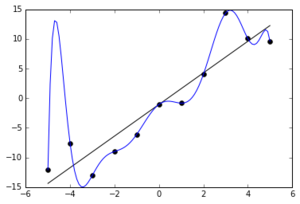
\includegraphics[width = 10cm]{Overfitted_Data.png}
    \caption{Overfitted function}
\end{figure}

Problem: We need to find a way to make the function depend on features which actually impact the target variable only, so that it does not try to overfit to noise using the remaining features. That is, the coefficients of features $x_m$ that are not required should go to $0$ in $h(\overrightarrow{x}) = w^T\overrightarrow{x}$.\\
Possible Solution: Penalise a norm of $w$ to decrease the number of non-zero values. So, $$loss = min_w \sum_{i \in D} (y_i-w^T\overrightarrow{x_i})^2 + \lambda \|w\|$$
\begin{flushleft}
Q. Which norm, $\|w\|_0, \|w\|_1, \|w\|_2$?\\
\color{blue}
If we want to encourage sparsity (few non-zero values in the vector $w$), ideally we should try to minimize $\|w\|_0$ which is the number of non-zero values in $w$. But it is not differentiable. So, it is not used.\\
Therefore we approximate it with $\|w\|_1$ because it encourages sparsity. If the true $w^*$ has only $k$ non-zero values where $k/dim(w) << 1$ then L1 regularization ($\|w\|_1$ minimization) will recover it almost surely (with probability 1).
\end{flushleft}


\section{Probabilistic Interpretation}

Now the question is what is the Probabilistic Interpretation of the regularized loss?
$$\min_w \sum_i (y_i - W^Tx_i)^2 + reg$$
Here reg is the regularization of from L1 norm or L2 norm.\\

Or we can also ask what is the equivalent MLE?

Say $D$ is data and $W$ is used to generate data.

$P(D|W)$ is the likelihood that data $D$ is generated by $W$ or the distribution of the data given a $W$

$P(W)$ is the likelihood that the $W$ we are using is correct $W$ or the Prior distribution of $W$\\


We want to maximize the likelihood of the distribution to recover the loss. i.e.

$$\max_W P(D|W)P(W)$$

Normally we used to assume that the $W$ is uniformly distributed and thus we use to only maximize the likelihood of the data given a $W$.

Now we assume that $W$ is a Gaussian distribution with parameter $\lambda$.

Suppose that $W \sim N(0,\sigma^2)$ then, $\lambda \propto \frac{1}{\sigma^2}$

\begin{flushleft}
Q. What is the significance of $\lambda$?\\
\color{blue}
As $\lambda \rightarrow high value \implies \sigma \rightarrow 0 \implies ||W|| \rightarrow 0$ as we are restricting the prior distribution of $W$. 
\end{flushleft}

\begin{flushleft}
Q. How to find a good value $\lambda$?\\
\color{blue}
\begin{enumerate}
    \item Find $W$ as a function of $\lambda$
    \item Test it on the validation set and find error as a function of $\lambda$ i.e. Error($\lambda$)
    \item Now minimize this error function and find the optimal $\lambda$ i.e. $\lambda^* = \min_\lambda \ Error(\lambda)$
\end{enumerate}
\end{flushleft}

Q. How error($\lambda$) vs $\lambda$ looks like?\\

\begin{figure}[h]
    \centering
    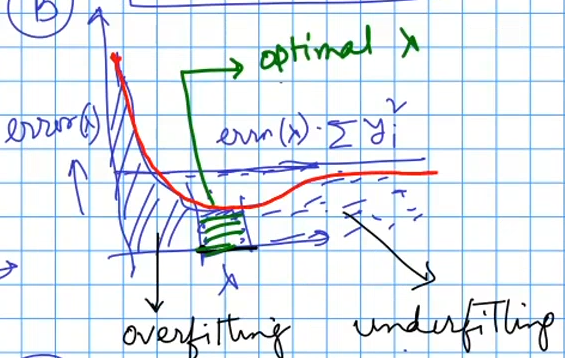
\includegraphics[width = 5.8cm]{Model complexity.png}
    \caption{error($\lambda$) vs $\lambda$}
\end{figure}
%----Covered till 62:41 in recording. Continue below this line-----------------------------------------
\section{Summary}
1.optimal value of mean squared loss minimization is-
$$ argmin_w \sum_{i \in D} (y_i- w^Tx_i)^2 + \lambda \|w\|^2$$

2.feature variable- $ \overrightarrow{x} = [x,\ x^2,\ x^3,\ \ldots,\ x^d]$
$$l_2 = min_w \sum_{i \in D} (y_i-w^T\overrightarrow{x_i})^2$$
For above problem,loss on the trainset is very low but loss on a testset is very high, this is called \textbf{Overfitting}\\
\\
3.Assuming W is a Gaussian distribution with parameter ($\lambda$), and $W \sim N(0,\sigma^2)$ then, $\lambda \propto \frac{1}{\sigma^2}$.\\
Significance of ($\lambda$), As $\lambda \rightarrow high value \implies \sigma \rightarrow 0 \implies ||W|| \rightarrow 0$ as we are restricting the prior distribution of $W$\\
\\
4.To find a good ($\lambda$), We find W as a function of ($\lambda$), find error by testing it on validation set and then minimize this error and find optimal ($\lambda$).\\
\\
5.Variation of Error($\lambda$) looks like Error tends to infinity when ($\lambda$) tends to 0,it then reaches a minimum value and when ($\lambda$) tends to infinity it reaches a finite value of $\sum_i (y_i)^2 $

\section{Group Details and Individual Contribution}
\begin{itemize}
    \item (19D070003) Adit Akarsh: Sections 6.1-6.2
    \item (190100007) Aditya Vijay Jain:  Section 6.3
    \item (200110064) Loveneesh Lawaniya: Section 6.3
    \item (200040106) Prateek Jha: Section 6.4
\end{itemize}



% Fill this part
\end{document}





